\section{Nuestra herramienta: }
\label{Implementacion}

	En esta sección se explica como se llevó a cabo la implementación de la solución
	propuesta en la Sección \ref{Solucion}, cumpliendo a su vez los objetivos
	planteados en la Sección \ref{Objective}. Para ello se desarrollaron dos
	herramientas:
	\emph{Pure Objects Observable} (POO) para atacar a la problemática de la
	observabilidad, y \emph{Pure Object Transaction} (POT) para atacar a la
	problemática transaccional.

\section{Nuestra herramienta: }

	En esta sección se explica como se llevó a cabo la implementación de la solución
	propuesta en la Sección \ref{sec:Solucion}, y cumpliendo el objetivo detallado
	en la Sección \ref{sec:Objetivo}. Se desarrollaron dos herramientas
	fundamentales para lo planteado. \emph{Pure Objects Observable} (POO) para atacar a la
	problemática de la observabilidad y \emph{Pure Object Transaction} (POT) para
	atacar a la problemática transaccional.
		
	\subsection{Selección de un framework de aspectos}  
		Un primer paso para la implementación de la herramienta fue la selección de una
		tecnología que permitiera desarrollar utilizando programación orientada a
		aspectos.
		Con ese objetivo, se evaluaron dos frameworks: Javassist \cite{??} y AspectJ
		\cite{KiczalesHHKPG01}.
		
		\medskip 
		Encontramos que AspectJ es una herramienta de más alto nivel, que extiende
		el lenguaje Java agregando construcciones específicas para trabajar con
		los conceptos de la teoría de programación orientada a aspectos.
		Por otro lado AspectJ requiere que el programador que use nuestro framework
		utilice un compilador específico. Consideramos que esta característica es muy
		negativa, por condicionar el entorno de trabajo de los usuarios de nuestra
		herramienta.
		En cambio Javassist agrega los aspectos al momento de la carga de las clases,
		sólo requiere que utilicemos un \emph{ClassLoader} específico.
		
		Elegimos Javassist por su menor impacto para el programador que utilice el
		framework como usuario.
		Para minimizar los problemas asociados a utilizar un framework de tan bajo
		nivel desarrollamos una herramienta que simplifica su uso agregando algunas
		abstracciones útiles. Esta herramienta se describe en la sección siguiente.

	\subsection{Desarrollo de Aspect for Pure Objects}

		El framework Javassist permite modificar directamente el \emph{bytecode} de
		una clase en el momento de cargarla.
		Por ser de tan bajo nivel es uno de los frameworks de aspectos más poderosos,
		pero a su vez el código se hace poco entendible.
		Por eso se desarrolló una herramienta llamada \emph{Aspect for Pure Objects} (APO), 
		que permite configurar aspectos utilizando conceptos de más alto nivel y
		aplicárselo a un grupo de objetos.
		
		La Figura \ref{aopImage} muestra esquemáticamente el diseño de la herramienta.
		Una instancia de \code{AdviceWeaver} se ocupa de aplicar los cambios sobre las
		clases.
		Para ello cuenta con un conjunto de \code{Advice} que consisten de un
		\code{Predicate} (que determina el conjunto de clases sobre el que aplica el
		advice) y un objeto que implemente la interfaz \code{ExprEditor} (que
		será el responsable de realizar las modificaciones sobre
		las clases alcanzadas por el advice).
		Finalmente una instancia de \code{APOClassLoader}, instalada como class loader
		del sistema permite que antes de utilizar cualquier clase esta pueda ser procesada por el \code{AdviceWeaver}
		
		Para implementar las modificaciones se provee una implementación de
		\code{ExprEditor} que contiene una colección de modificaciones expresadas en un
		lenguaje de alto nivel y las traduce al lenguaje de bajo nivel que requiere el
		framework Javassist.
		La Figura \ref{pooCode} muestra un ejemplo de código de este lenguaje de alto nivel,
		tomado del framework POO, que se describe en la Sección \ref{poo}.
		
		\begin{figure}[h]
			\centering
			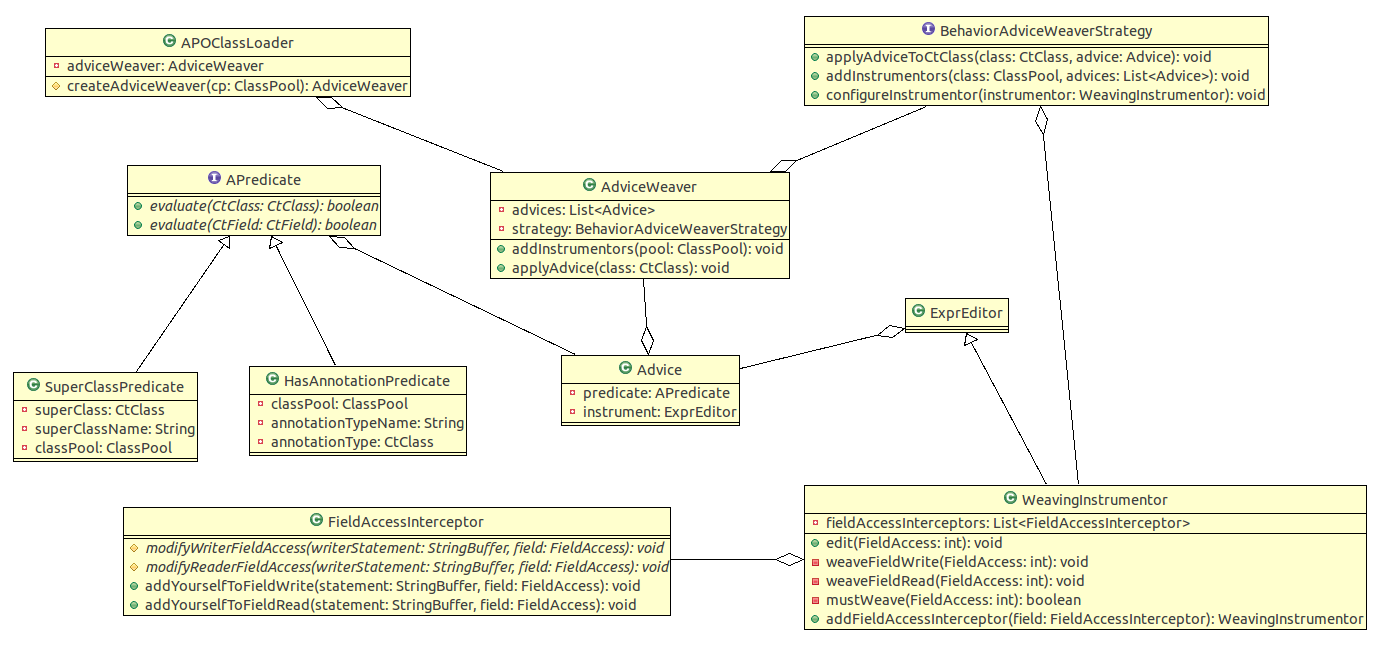
\includegraphics[width=500px, height=500px]{img/aop}
			\caption{Diagrama UML de la herramienta APO}
			\label{aopImage}
		\end{figure}	 
		
		
		A su vez, la Tabla \ref{table} describe las expresiones propias del lenguaje
		definido por APO, su traducción al lenguaje de expresiones de
		Javassist y su significado.
		
		\begin{figure}[h]
			\begin{lstlisting}
	$Object oldValue = $oldValue;
	$originalAsigment;
	$this.firePropertyChange('$fieldName', oldValue, $newValue);
			\end{lstlisting}
			\caption{Fragmento de código del framework POO}
			\label{pooCode}
		\end{figure}
		
		\begin{table}[h]
			\begin{tabular}{|+l^l^p{7cm}|}
				\hline
				\rowstyle{\bfseries}%
					Expr. APO & Expr. Javassist & Significado \\
				\hline
					\$Object & java.lang.Object & El nombre completo de la clase Object \\
				\hline
					\$this & \$0 & El objeto receptor del mensage.\\
				\hline
					\$newValue & \$1 & El primer parametro del método. \\
				\hline
					\$oldValue &  \$0.getAtribute() & El valor del atributo antes de
				la asignación que está siendo modificada.\\
				\hline
					\$originalAsigment & \$0.atribute = \$1 & La asignación del atributo con el
				primer parametro del método.\\
				\hline
					``\$fieldName'' & ``atribute'' & El nombre del atributo como un String.\\
				\hline
			\end{tabular} 
			\caption{Tabla de equivalencia {explicar ``atribute''}}
			\label{table}
		\end{table}

\emph{Pure Object Transaction} (POT) es la herramienta que implementa el
aspecto transaccional definido en la sección \ref{aspectoTransaccional}.
Está basada en una implementación anterior de Nicolás Passerini y Javier
Fernandes, que se actualizó para aprovechar el framework APO y facilitar su
integración con las demás herramientas desarrolladas.

\medskip
 
Este framework intercepta todas las lecturas y escrituras de los atributos de
un objeto, delegando tanto las lecturas como las escrituras al
\emph{administrador de las transacciones}.
A su vez, el administrador de transacciones asocia el pedido con un contexto
transaccional, que guarda los valores de los atributos de un objeto que fueron
modificados durante la transacción en una estructura de la forma
\code{[objeto, [nombre del atributo, valor]]}.
Cada contexto transaccional esta asociado a un \emph{thread}. Esto
permite manejar la concurrencia en el acceso a la información de los objetos.
Para aplicarle este aspecto a una clase se utiliza la \emph{annotation} \lstinline|Transactional| como
se muestra en la Figura \ref{annoTransactional}.

\begin{figure}[hbt]
	\begin{lstlisting} 
		@Transactional
		public class Account {
		}
	\end{lstlisting}
	\caption{Annotation para aplicar el aspecto transaccional.}
	\label{annoTransactional}
\end{figure}
	
\medskip
 
La herramienta provee también soporte para transacciones anidadas.
Al momento de hacer el \emph{commit} en una transacción, los valores
contenidos en el contexto transaccional son impactados en la transacción
padre.
En caso de tratarse de una transacción de primer nivel, los cambios se impactan
en los objetos de dominio usando \emph{reflection}.
Esta forma de implementación permite que la identidad del objeto se
mantenga, ya que el objeto no se modifica ni se clona, solo se intercepta el
acceso a sus atributos.

Otro agregado a la versión original es la intersección de las modificaciones 
a un objeto de tipo \lstinline|Collection|, por ejemplo agregar o quitar
objetos de una colección.
Esto presenta un desafío especial ya que habitualmente en los programas Java
se utilizan las implementaciones de colecciones provistas por el propio
lenguaje y no es posible aplicar aspectos sobre estas clases. 
En la nueva versión, este problema se resuelve reemplazando en forma
automática las colecciones del lenguaje Java por
implementaciones propias de las mismas interfaces.
La figura \ref{potuml} muestra esquemáticamente el diseño de la herramienta.

\begin{figure}[hbt]
	\centering
	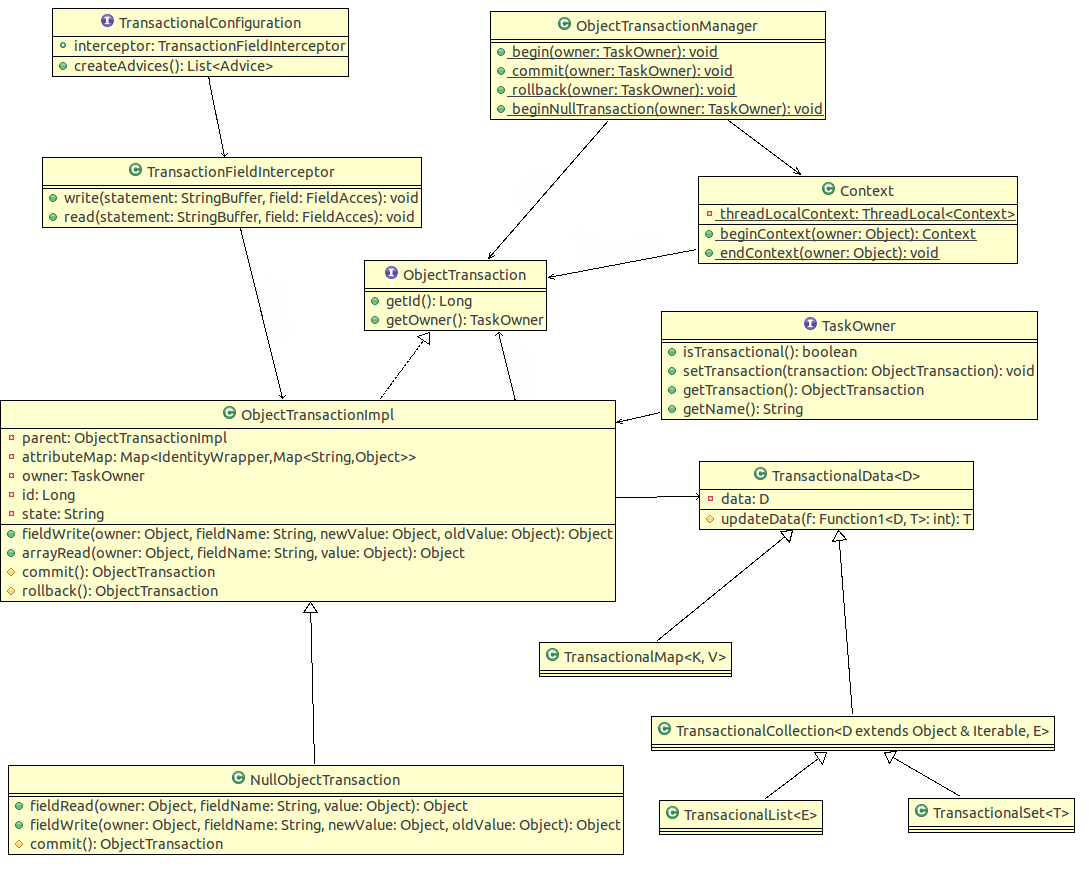
\includegraphics[scale=0.4]{img/pot}
 	\caption{Esquema de la herramienta POT}
 	\label{potuml}
\end{figure}

\subsection{Pure Observable Objects}
	\label{poo}
	Pure Observable Objects (POO) es el framework que implementa el
	aspecto Observable planteado en la Sección \ref{aspectoObservable}.
	La implementación interna del aspecto agrega un
	atributo llamado \lstinline|changeSupport| del tipo
	\lstinline|PropertySupport| al objeto al que se le aplica el aspecto.
	\lstinline|PropertySupport| es una interfaz, la implementación concreta a
	utilizar se obtiene del el archivo de configuración.
	
	Para completar el objetivo se agregan los métodos 
	\lstinline|addPropertyChangeListener| y
	\lstinline|removePropertyChangeListener| que permiten agregar 
	y remover observadores, y \lstinline|firePropertyChange|
	que notifica a los observadores que un atributo ha cambiado.
	
	Para entender mejor el modelo de classes, la la figura \ref{fig:poo} muesta
	esquemáticamente el diseño de la herramienta.
	
	\begin{figure}
		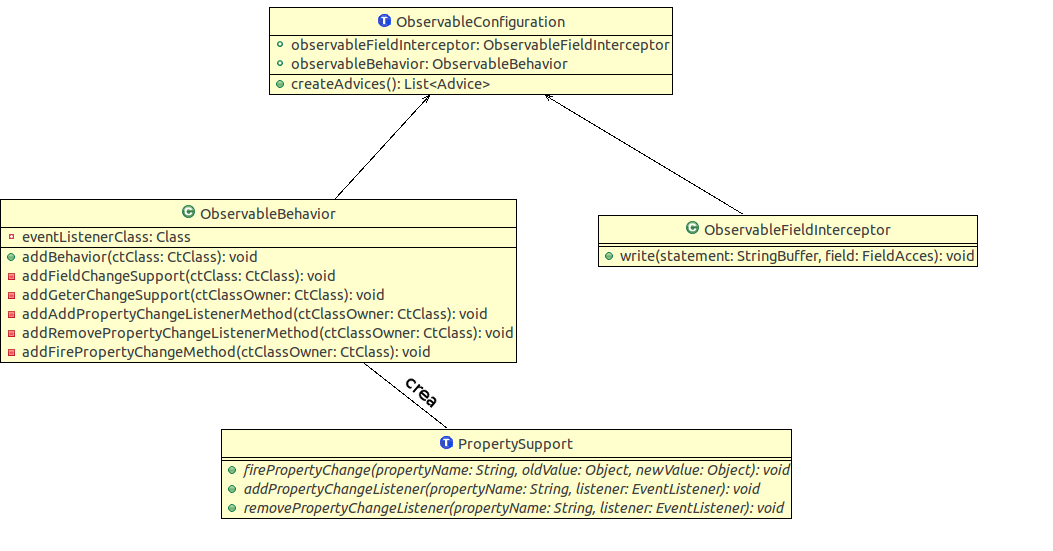
\includegraphics[width=450px, height=200px]{img/poo}
	 	\label{fig:poo}
	 	\caption{}
	\end{figure}
	
	Para agregarle este aspecto a una clase se utiliza la \emph{Annotation}
	\lstinline|Observable|.
	
	\begin{lstlisting} 
		@Observable
		public class Client{
		}
	\end{lstlisting}

\subsection{Integración de POT, POO y Arena}
La integración entre Arena y POO se realizó construyendo una implementación de
\lstinline|PropertySupport| que dispara los eventos de acuerdo a los esperado
por el framework Arena.

\medskip
Por otro lado, la clase \lstinline|TransactionalDialog| permite integrar Arena y
POT.
Definir una ventana como una subclase de
\lstinline|TransactionalDialog| asocia automáticamente a esa ventana con un
contexto transaccional.
Al abrirse la ventana se efectúa la operación de \emph{beginTransaction}.
Luego, botones \emph{Aceptar} y \emph{Cancelar} (que por defecto son agregados
por la superclase) efectúan las acciones de \emph{commit} y
\emph{rollback}.

\medskip
En tercer lugar, como se explicó en la sección \ref{sec:Union}, para integrar
los dos aspectos entre sí se requiere filtrar los eventos disparados por los objetos de dominio, 
limitándolos a las ventanas que se encuentran dentro del mismo contexto
transaccional. 
Se implementaron tres niveles de aislamiento de los eventos:
\begin{description}
	\item[\emph{Fire All}] Todos los eventos disparados por el dominio son
	escuchados, sin importar si están en un transacción.

	\item[\emph{Fire Committed}] Solo se escucha los eventos de las transacciones
		comiteadas
	
	\item[\emph{Fire olnly in my transaction}] solo se escucha los eventos que
		ocurren dentro de su translación.
 \end{description}
 
\medskip
Finalmente, el framework se puede configurar para utilizar uno, otro o ambos
aspectos, según se requiera.
Los objetos pueden ser anotados con \emph{Observable} y
\emph{Transactional} como vimos previamente, 
o bien utilizar \emph{TransactionalAndObservable} que es una unión de ambas.

	\begin{lstlisting} 
		@TransactionalAndObservable
		public class Client{
		}
	\end{lstlisting}

\subsection{Otras mejoras al Arena}
	La integración se realizo con el lenguaje de programación Scala
	\cite{OderskySpoonVenners08}. Para llevar al cabo la integración fue necesario agregar algunas
	mejoras en Arena:
	\begin{description}

	  \item[Bindings anidados] Como se vio en la Sección \ref{binding},
		  el \emph{binding} es una conección de propiedades entre dos objetos. Con
		  esta idea se desarrolló un tipo de binding que permite conectar propiedades
		  anidadas entre dos objetos, por ejemplo,  la figura \ref{bindAnidado}

			\begin{figure}[h]
			\centering
					\begin{lstlisting}
						bindProperty("source.owner.name	") 
					\end{lstlisting}
			\caption{Ejemplo de binding de con la Clase Transaction}
			\label{bindAnidado}
		\end{figure}	

	  \item[Monitor de Transacciones]
		 Se desarrolló un \emph{Monitor de Transacciones}, que permite
		 \emph{debuggear} las transacciones abiertas actualmente, mostrando
		 los objetos afectados por la transacción y los atributos que se
		 modificaron.
		La figura \ref{monitor} muestra el monitor de transacciones\ldots
		
		\begin{figure}[h]
			\centering
			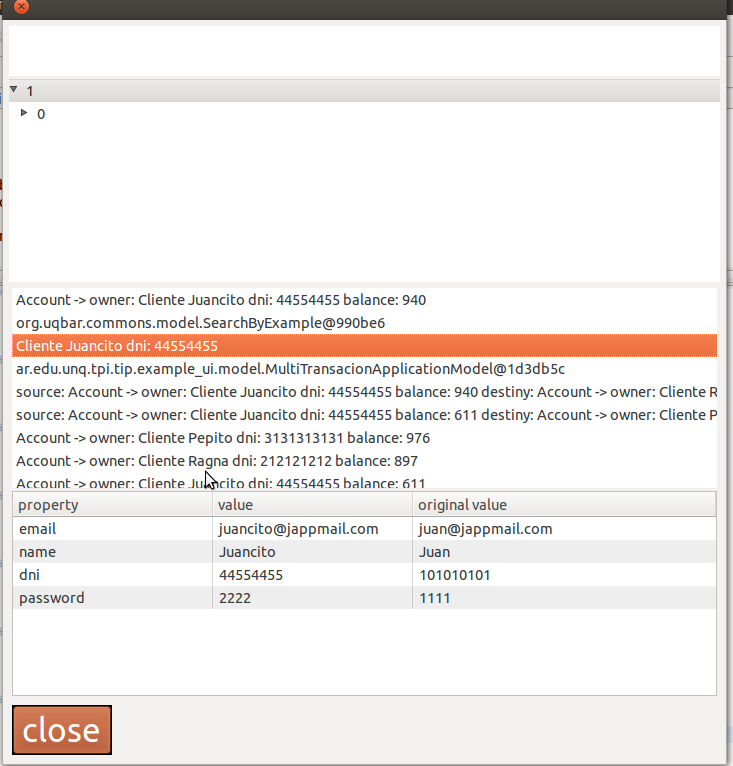
\includegraphics[width=430px, height=480px]{img/monitorTransacciones.png}
			\caption{Monitor}
			\label{monitor}
		\end{figure}	
	
	  \item[Nuevos componentes] Se agregaron algunas estructuras visuales como
	  arboles y listas.
	\end{description}

\section{Aplicación de ejemplo}
Para ilustrar el uso de las herramientas desarrolladas utilizaremos como ejemplo
una aplicación bancaria, en la que los clientes de un banco pueden transferir
dinero de una cuenta a otra. 
Realizar una transferencia implica extraer de una cuenta el
monto indicado, y depositarlo en otra. 
En cualquiera de los dos pasos de la transferencia (extraer y depositar) se
pueden producir errores.
Por ejemplo, el saldo puede ser insuficiente o el depósito puede superar el
máximo permitido.
La figura \ref{example} muestra las clases que implementan la lógica del
dominio.

	\begin{figure}[h!]
		\centering
		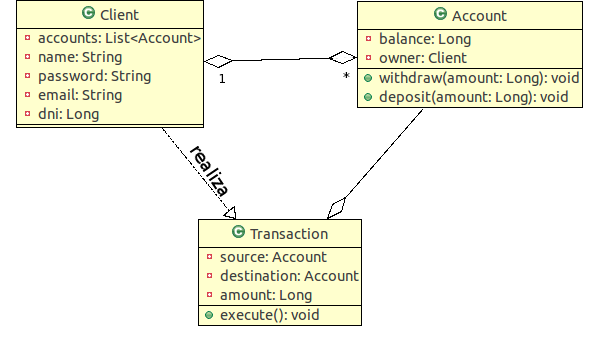
\includegraphics[width=450px, height=250px]{img/transaccion}
		\caption{Diagrama UML de la aplicación de ejemplo}
		\label{example}
	\end{figure}	

A continuación se describirán las dos pantallas más importantes de la
aplicación, que nos permitirán mostrar las diferentes utilidades brindadas por
nuestra herramienta.
 
\begin{description}

	\item[Pantalla de Transferencia Simple]
		Esta primera pantalla permite elegir una de las cuentas propias, otra cuenta
		de cualquier otro cliente del sistema y realizar una transferencia de la
		primera hacia la segunda con el monto indicado. Esta pantalla se
		muestra en la figura \ref{trasferenciaSimple}.
		
		\begin{figure}[h]
			\centering
			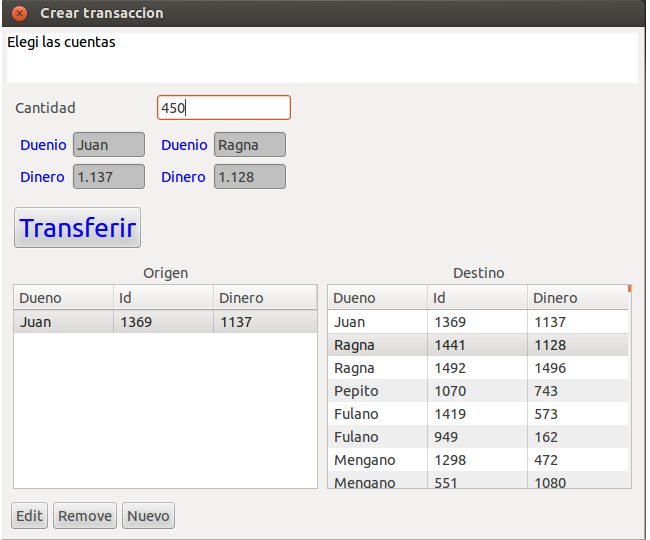
\includegraphics[width=450px, height=375px]{img/simple-transferencia}
			\caption{Pantalla de transferencia}
			\label{trasferenciaSimple}
		\end{figure}

		Desarrollar esta utilidad con nuestra herramienta nos permite que el código
		solo se concentre en lo importante, que es debitar y extraer el monto. %Manejo de errores
		La figura \ref{executeTransaction} muestra el método  \lstinline|execute| de la
		clase \lstinline|Transaction| 
		Dado que código de dominio es limpio, no hay comportamiento fuera de la logica
		de negocio que pueda provocar un error.

		\begin{figure}[h]
			\begin{lstlisting}
				public void execute(){
					this.source.withdraw(this.amount);
					this.destination.deposit(this.amount);
				}
			\end{lstlisting}
			\caption{Fragmento de código de la Clase Transaction}
			\label{executeTransaction}
		\end{figure}
		 
		
	\item[Pantalla de Transferencias Múltiples]
		Esta segunda pantalla nos permite realizar multiples transferencias
		simultáneamente.
		Estas transferencias pueden ser confirmadas o canceladas en su todalidad en
		cualquier momento.
		A diferencia de la transferencia simple, se agrega una
		lista con las transferencias que se llevan a cabo.
	
		\begin{figure}[h]
			\centering
			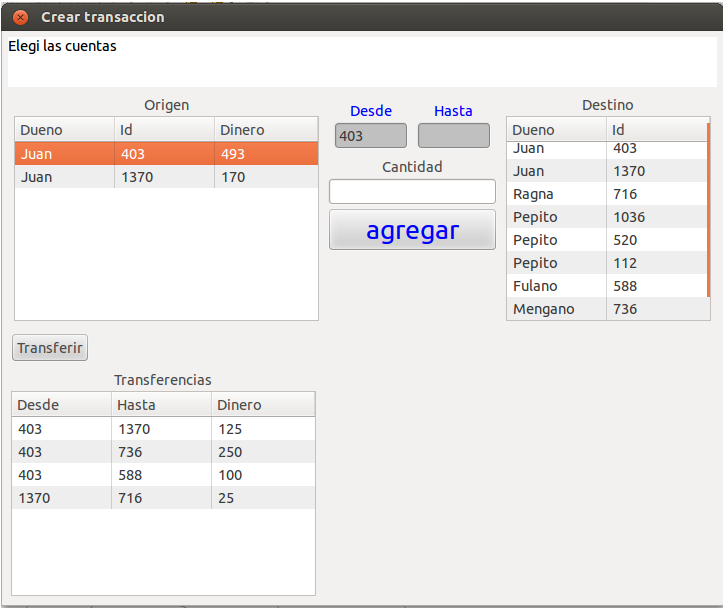
\includegraphics[width=450px, height=380px]{img/multTransferencias}
			\caption{Pantalla de transferencia}
			\label{trasferenciaMultiple}
		\end{figure}
		
\end{description}